% !TeX program = pdflatex
\documentclass[tikz,border=8pt]{standalone}
\usepackage{tikz}
\usetikzlibrary{calc}
\definecolor{FigureBlue}{HTML}{2563EB}
\definecolor{FigureOrange}{HTML}{EA580C}
\definecolor{FigureSlate}{HTML}{64748B}
\begin{document}
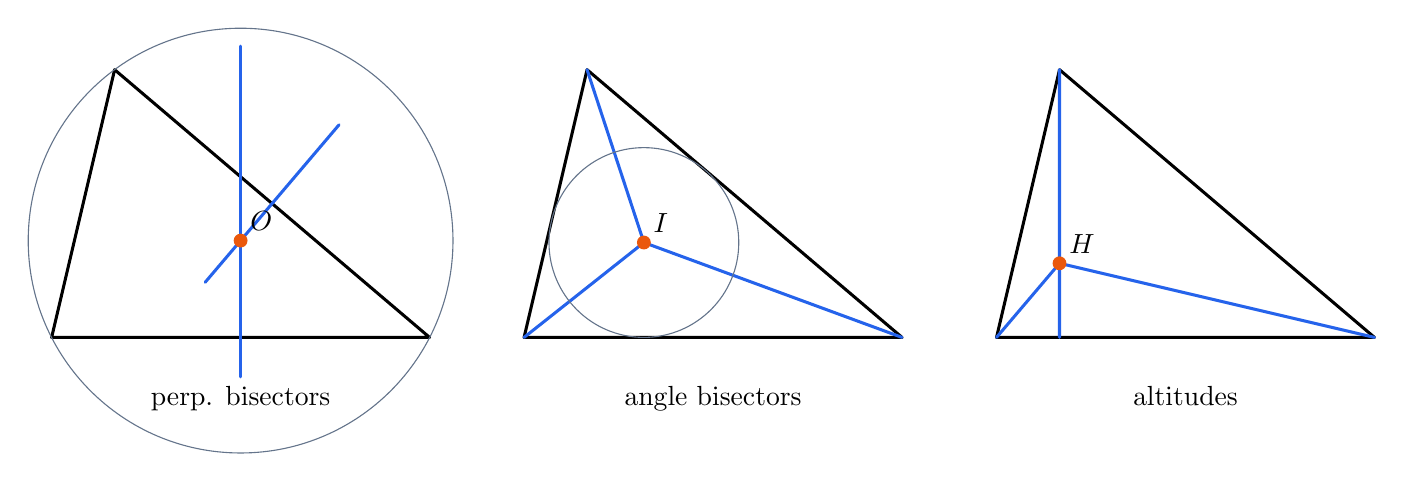
\begin{tikzpicture}[line cap=round,line join=round]
  \begin{scope}
    \coordinate (A) at (.8,3.4); \coordinate (B) at (0,0); \coordinate (C) at (4.8,0);
    \coordinate (O) at (2.4,1.2294118);
    \coordinate (Mbc) at (2.4,0); \coordinate (Mca) at (2.8,1.7);
    \draw[line width=1.1pt] (A)--(B)--(C)--cycle;
    \draw[FigureBlue,line width=1.1pt] (2.4,-.5)--(2.4,3.7);
    \draw[FigureBlue,line width=1.1pt] ($(Mca)-(.85,1)$)--($(Mca)+(.85,1)$);
    \draw[FigureSlate] (O) circle[radius=2.6972];
    \fill[FigureOrange] (O) circle (2.5pt); \node[above right] at (O) {$O$};
    \node[below=5mm] at (Mbc) {perp. bisectors};
  \end{scope}
  \begin{scope}[xshift=6cm]
    \coordinate (A) at (.8,3.4); \coordinate (B) at (0,0); \coordinate (C) at (4.8,0);
    \coordinate (I) at (1.52154,1.20510);
    \draw[line width=1.1pt] (A)--(B)--(C)--cycle;
    \draw[FigureBlue,line width=1.1pt] (A)--(I) (B)--(I) (C)--(I);
    \draw[FigureSlate] (I) circle[radius=1.20510];
    \fill[FigureOrange] (I) circle (2.5pt); \node[above right] at (I) {$I$};
    \node[below=5mm] at ($(B)!.5!(C)$) {angle bisectors};
  \end{scope}
  \begin{scope}[xshift=12cm]
    \coordinate (A) at (.8,3.4); \coordinate (B) at (0,0); \coordinate (C) at (4.8,0);
    \coordinate (H) at (.8,.9411765);
    \draw[line width=1.1pt] (A)--(B)--(C)--cycle;
    \draw[FigureBlue,line width=1.1pt] (A)--(.8,0) (B)--(H) (C)--(H);
    \fill[FigureOrange] (H) circle (2.5pt); \node[above right] at (H) {$H$};
    \node[below=5mm] at ($(B)!.5!(C)$) {altitudes};
  \end{scope}
\end{tikzpicture}
\end{document}
